% !TEX program = XeLaTeX
% !TEX encoding = UTF-8
\documentclass[utf8,nofonts]{article}
%{ctexart}


%\setCJKmainfont[BoldFont=FandolSong-Bold.otf,ItalicFont=FandolKai-Regular.otf]{FandolSong-Regular.otf}
%\setCJKsansfont[BoldFont=FandolHei-Bold.otf]{FandolHei-Regular.otf}
%\setCJKmonofont{FandolFang-Regular.otf}

\usepackage[utf8x]{inputenc}
\usepackage[russian]{babel}    %% 3

\usepackage{url}
\usepackage{cancel}
\usepackage{xspace}
\usepackage{graphicx}
\usepackage{multicol}
\usepackage{multirow}
\usepackage{subfig}
\usepackage{amsmath}
\usepackage{amssymb}
\usepackage[a4paper, width=186mm, top=18mm, bottom=18mm, includeheadfoot]{geometry}
%\usepackage[a4paper, width=140mm, top=18mm, bottom=22mm, includeheadfoot]{geometry}
\usepackage{booktabs}
\usepackage{array}
\usepackage{verbatim}
\usepackage{caption}
\usepackage{natbib}
\usepackage{booktabs}
\usepackage{float}
\usepackage{pdflscape}
\usepackage{mathtools}
\usepackage[usenames, dvipsnames]{xcolor}
\usepackage{afterpage}
\usepackage{pgf}
\usepackage{tikz}
\usepackage{dirtree}
\usepackage[style=american]{csquotes}
\usepackage{amsfonts}
\usepackage{tikz}
\usepackage{tkz-graph}
\usetikzlibrary{arrows,decorations.pathmorphing,automata,positioning,backgrounds,fit,shapes.symbols,chains,intersections}

\newtheorem{definition}{Definition}[section]
\newtheorem{theorem}{Theorem}[section]
\newtheorem{lemma}{Lemma}
\newtheorem{proof}{Proof} [section]



\usepackage[toc, page, title, titletoc, header]{appendix}
\usepackage{marginnote}
\usepackage{tablefootnote}

\renewcommand\appendixname{Приложения}



\usepackage{perpage} %the perpage package
\MakePerPage{footnote} %the perpage package command

\usetikzlibrary{shapes.geometric}%
\usepackage{color}
%\usepackage[pages=some, placement=top]{background}
\usepackage{eso-pic}
\usepackage[final]{pdfpages}

%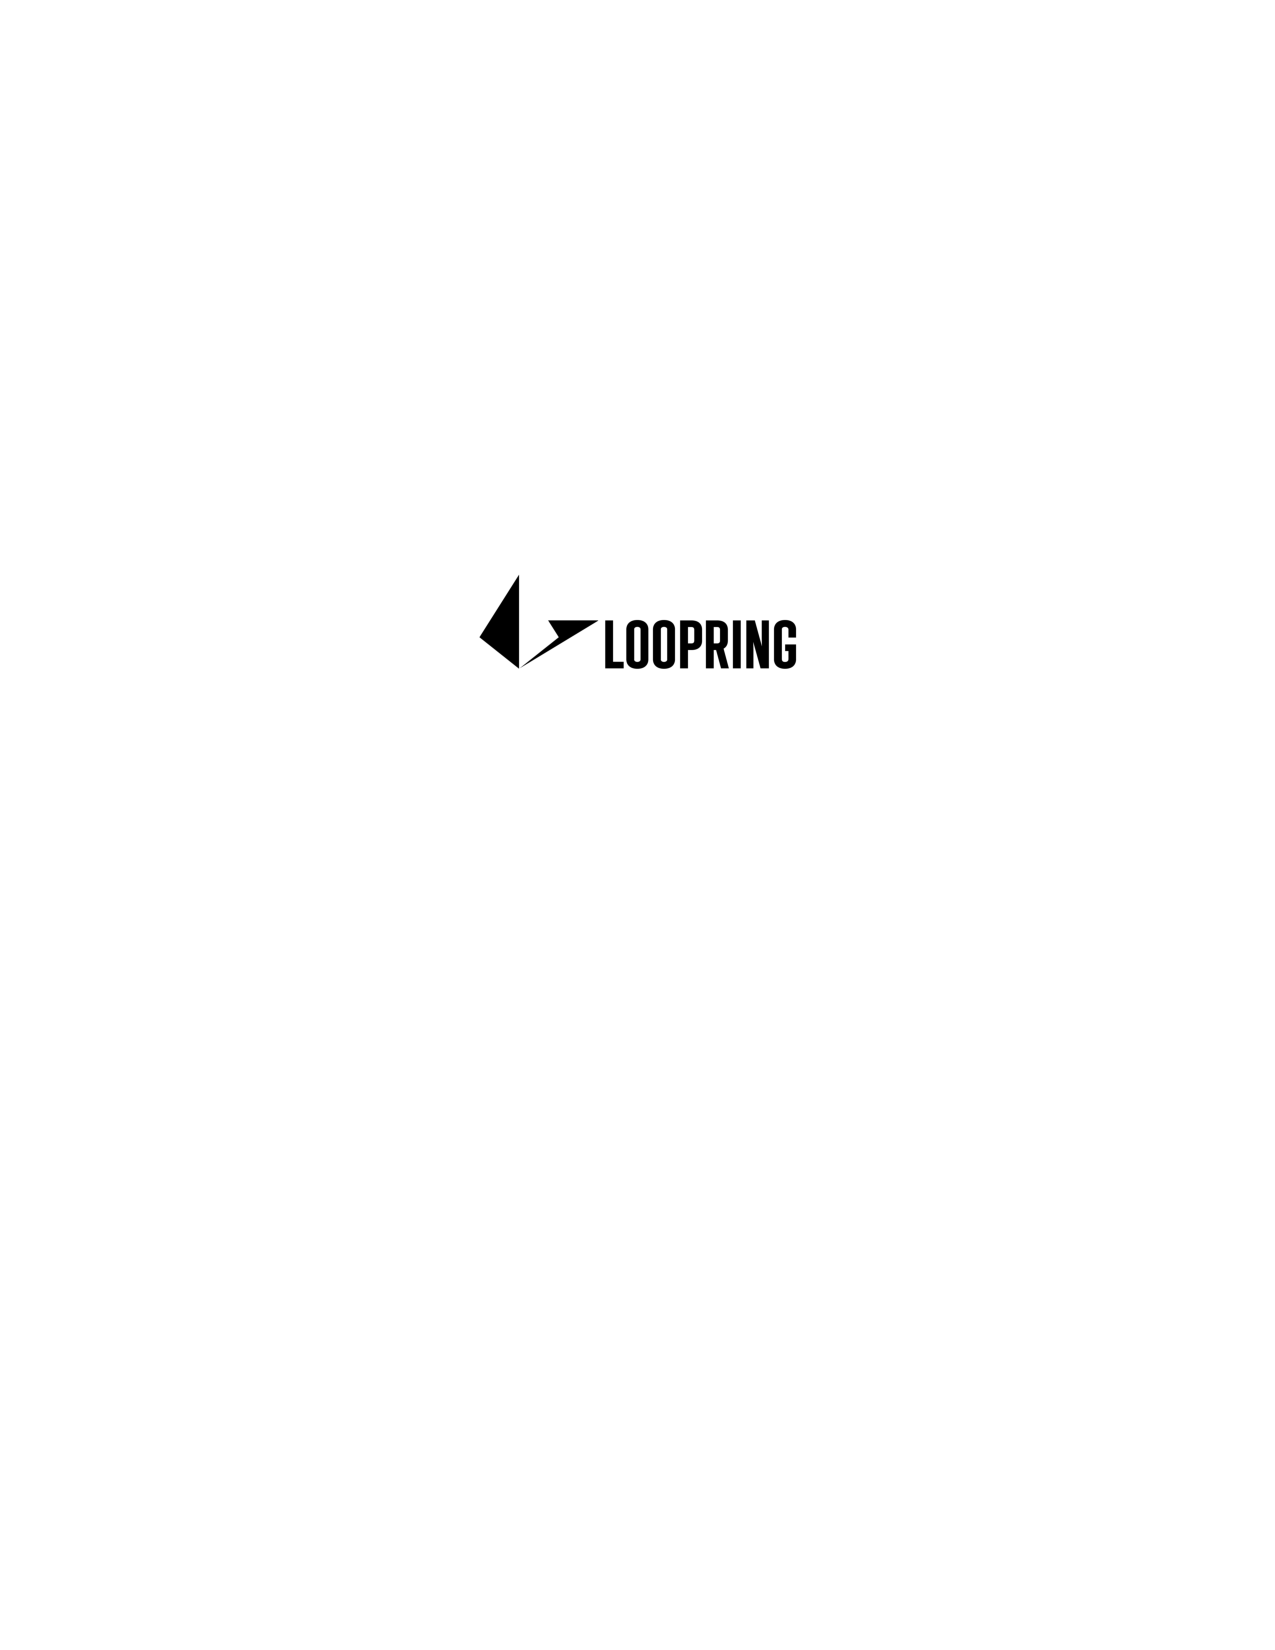
\includepdf[pages=1]{cover}
\hyphenpenalty=750

\title{\textbf{Loopring:}\\\textbf{Децентрализованный протокол обмена}}
\author{
  Daniel Wang\\
  \texttt{daniel@loopring.org}\\
  \and
  	Jay Zhou\\
  	\texttt{jay@loopring.org}\\
  	\and
  	Alex Wang\\
  	\texttt{alex@loopring.org}\\
  	\and
  	Matthew Finestone\\
  	\texttt{matt.finestone@gmail.com}\\ 
  \\
  \texttt{https://loopring.org}
 }

\makeatletter
\def\CTEX@section@format{\Large\bfseries}
\makeatother

\makeatletter
\newenvironment{tablehere}
 {\def\@captype{table}}
 {}

\newenvironment{figurehere}
 {\def\@captype{figure}}
 {}
\makeatother



\begin{document}
%\AddToShipoutPicture{\BackgroundPic}
\maketitle


\begin{abstract}
	Loopring - открытый протокол для создания децентрализованных бирж. Loopring работает как набор смарт контрактов, ответственных за торговлю и взаиморасчеты, причем объединение и передача ордеров происходит офчейн. Протокол является бесплатным, расширяемым и служит стандартным строительным блоком для децентрализованных приложений (dApps), которые включают функциональные возможности обмена. Его совместимые стандарты способствуют анонимной торговле. Важным улучшением по сравнению с существующими децентрализованными протоколами обмена является способность ордеров смешиваться и взаимодействовать с другими ордерами, устраняя ограничения торговых пар и резко увеличивая ликвидность. Loopring также использует уникальное и надежное решение для предотвращения опережающей сделки: невозможно отправить транзакции в блок быстрее, чем это сделает валидный узел. Loopring является блокчейн независимым и развертывается на любом блокчейне, поддерживающем смарт контракты. На момент написания статьи он работает на Ethereum \cite{buterin2017ethereum} \cite{wood2014ethereum}, а Qtum \cite{dai2017smart} и NEO \cite{atterlonn2018distributed} на стадии разработки.
\end{abstract}



\begin{multicols}{2}
	\section{Введение\label{sec:introduction}}
	
	С ростом количества активов на базе блокчейнов значительно увеличилась потребность в обмене этими активами между пользователями. По мере ввода новых токенов, включая токенизацию традиционных активов, эта потребность будет только увеличиваться. Если исключить спекулятивную составляющую торговли, возможность обмена одной криптовалюты на другую является основополагающей для более крупной экосистемы. Действительно, в криптовалютах есть скрытый потенциал \cite{desotocapital}, который полностью можно раскрыть лишь с возможностью свободно передавать и преобразовывать эти активы. 
	
	Таким образом, надежный обмен токенами является обязательным для технологии блокчейн. Однако до сих пор крипто-энтузиасты в основном торговали токенами на традиционных централизованных биржах. Протокол Loopring необходим, потому что, как отмечено еще в Биткойн \cite{nakamoto2008bitcoin}, что в отношении электронных денег \enquote{основные преимущества теряются, если третья сторона по-прежнему нуждается в предотвращении двойных расходов}, поэтому основные преимущества децентрализованных активов также исчезают, когда они должны проходить через закрытые, централизованные биржи.  
	
	Торговля токенами на централизованных биржах не имеет смысла, поскольку они не поддерживают преимущества, которыми пользуются соответствующие децентрализованные проекты. Существуют также многочисленные риски и ограничения при использовании централизованных бирж, которые описаны ниже. Децентрализованные биржи (DEXs) \cite{schuh2015bitshares} \cite{bancor} \cite{kyber} попытались решить эти проблемы и, во многих случаях, преуспели в уменьшении рисков безопасности, используя блокировки. Однако, поскольку DEX становятся ключевым элементом для новой экономики, есть значительные возможности для повышения эффективности. Loopring стремится предоставить модульные инструменты для децентрализованных бирж с его открытым протоколом, не зависящем от dApp.
	
	\section{Обзор существующих бирж\label{sec:current_exchange_landscape}}
	
	\subsection{Недостатки централизованных бирж}
	Три основных недостатка централизованных бирж; 1) Отсутствие безопасности, 2) Отсутствие прозрачности и 3) Отсутствие ликвидности.
	
	\textbf{Отсутствие безопасности} возникает из-за того, что пользователи обычно делегируют контроль за своими секретными ключами одному централизованному объекту. Таким образом, появляется возможность того, что централизованные биржи станут жертвами хакеров. Безопасность и риски хакерских атак, с которыми сталкиваются все централизованные биржи, хорошо известны \cite{coincheckhack}  \cite{mcmillan2014inside}, но часто воспринимаются в качестве \enquote{вынужденных рисков} ради торговли токенами. Централизованные биржи по-прежнему являются лакомым куском для хакеров, поскольку их сервера хранят более миллиона долларов средств пользователей. Разработчики бирж также могут делать случайные ошибки в коде, от которых никто не застрахован. И самое главное, что пользователи не контролируют свои токены, когда они депонированы на централизованной бирже.
	
	\textbf{Отсутствие прозрачности} подвергает пользователей риску наткнуться на мошенническую биржу. Различие здесь заключается в малейших намерениях биржевого оператора, поскольку пользователи по-настоящему не владеют своими собственными активами на централизованных биржах, а скорее имеют особый вид долговой расписки. Когда токены отправляются на кошелек биржи, она берет их на хранение и предлагает долговую расписку. Таким образом, все сделки производятся между долговыми расписками пользователей. Когда пользователи погашают свои долговые расписки перед биржей, получают токены обратно на свой внешний кошелек. Во всем этом процессе отсутствует прозрачность, и биржа может закрыть, заморозить вашу учетную запись, обанкротиться и т. д. Также возможно, что они используют активы пользователя для других целей во время хранения, например, выдавая их третьим лицам. Отсутствие прозрачности может стоить пользователям как полной потери средств, так и более высокие комиссионные сборы, задержки, регуляторные риски и неисполненные ордера.
	
	\textbf{Отсутствие ликвидности.} С точки зрения биржевых операторов фрагментированная ликвидность препятствует появлению новых бирж из-за двух сценариев «победитель забирает все». Во-первых, выигрывает биржа с наибольшим количеством торговых пар, потому что пользователи считают, что желательно проводить все свои сделки на одной бирже. Во-вторых, выигрывает биржа с большей книгой заказов из-за благоприятных спрэдов между спросом и предложением для каждой торговой пары. Это препятствует конкуренции со стороны новичков, потому что им сложно создать первоначальную ликвидность. В результате многие биржи удерживают высокую долю рынка, несмотря на жалобы пользователей и даже серьезные инциденты с хакерами. Стоит отметить, что, поскольку централизованные биржи занимают большую долю на рынке, они становятся все более привлекательной целью для взлома.
	
	С точки зрения пользователей, фрагментированная ликвидность значительно снижает удобство. В централизованной бирже пользователи могут торговать только в собственных пулах ликвидности биржи, по собственной книге заказов и между поддерживаемыми парами токенов. Для обмена токена \verb|A| на токен \verb|B| пользователи должны пойти на биржу, которая поддерживает оба токена или регистрироваться на разных биржах, раскрывая личную информацию. Пользователям часто приходится выполнять предварительные или промежуточные сделки, как правило, в паре с BTC или ETH, оплачивая спреды в процессе обмена. Наконец, книги заказов могут быть недостаточно глубокими, чтобы завершить торговлю без изменения цены. Даже если биржа претендует на обработку больших объемов, нет никакой гарантии, что этот объем и ликвидность не являются поддельными \cite{fakevolume}.
	
	Результатом этого являются пробои ликвидности и фрагментированная экосистема, которая напоминает классическую финансовую систему, при этом значительный объем торговли централизован на нескольких биржах. Обещания ликвидности блокчейнов не имеют смысла в рамках централизованных бирж.
	
	\subsection{Недостатки децентрализованных бирж}
	Децентрализованные биржи отличаются от централизованных отчасти тем, что пользователи контролируют свои секретные ключи (активы) и совершают сделки непосредственно на основном блокчейне. Они успешно уменьшают многие из вышеперечисленных рисков, связанных с безопасностью. Однако проблемы сохраняются в отношении производительности и структурных ограничений. 
	
	Ликвидность зачастую остается проблемой, поскольку пользователи должны искать контрагентов через разрозненные пулы ликвидности. Эффекты фрагментированной ликвидности присутствуют, если DEX или dApps не используют согласованные стандарты для взаимодействия, и если ордера не распространяются на большую сеть. Ликвидность списков лимитных ордеров и, в частности, их отказоустойчивость -- как быстро заполненные лимитные ордера восстанавливаются -- могут существенно повлиять на оптимальные торговые стратегии \cite{limitorderliquidity}. Отсутствие таких стандартов привело не только к уменьшению ликвидности, но и к воздействию множества потенциально небезопасных проприетарных смарт контрактов.
	
	Кроме того, поскольку сделки производятся на блокчейне, DEXs наследуют ограничения этого блокчейна, а именно: масштабируемость, задержки в выполнении (майнинг) и дорогостоящие изменения ордеров. Таким образом, книга заказов блокчейна не очень хорошо масштабируется, так как выполнение кода на блокчейне затратно (газ), что делает несколько отмененных ордеров весьма дорогостоящей операцией. 
	
	Наконец, поскольку списки ордеров являются общедоступными, транзакция по размещению ордера видна майнерам, поскольку она ожидает, что ее добавят в следующий блок и только после этого помещают в список ордеров. Эта задержка подвергает пользователя риску оказаться не у дел, когда его ордер никогда не исполнится.
	
	\subsection{Гибридные решения}
	По вышеуказанным причинам основанные на блокчейне биржи имеют ограничения, которые делают их неконкурентоспособными по сравнению с централизованными биржами. Существует компромисс между ончейн операциями, централизованными биржами и гибкостью ордеров. Протоколы, такие как Loopring и 0x \cite{warren20170x}, совмещают возможности ончейн операций с офчейн управлением ордерами. Эти решения реализованы в открытых смарт контрактах, что ограничивает возможности масштабирования, выполняя несколько функций офчейн и предоставляя узлам гибкость при выполнении критических ролей для сети. Однако и в гибридной модели остаются недостатки \cite {costofdecent}. Протокол Loopring предлагает значимые различия в подходе к гибридному решению, описанные в этой статье.
	
	
	\section{Протокол Loopring\label{sec:loopring_protocol}}
	Loopring - это не DEX, а модульный протокол для построения DEX для нескольких блокчейнов. Мы разбираем на составные части традиционную биржу и предлагаем вместо нее набор открытых смарт контрактов и децентрализованных участников. Роли в сети делятся на кошельки, ретрансляторы, консорциум блокчейнов, разделяющих ликвидность, обозреватели списков ордеров, майнеров и сервисы токенизации активов. Перед определением каждого из них мы должны сначала разобраться с ордерами в Loopring. 
	
	\subsection{Кольцевой ордер\label{sec:order_ring}}
	Ордера в Loopring представляют собой так называемые Unidirectional Order Model (UDOM) \cite{coinport2014udom}. UDOM представляет ордер как запрос на обмен токенов, \verb|amountS|/\verb|amountB|, (сумма для продажи/покупки) вместо цен спроса и предложения. Поскольку каждый ордер является всего лишь обменным курсом между двумя токенами, отличительной особенностью протокола является смешивание и сопоставление нескольких ордеров в кольцевой ордер. Используя до 16 ордеров вместо одной торговой пары, имеем резкое увеличение ликвидности и потенциал для выравнивания цен. 
	
	\begin{center}
		\begin{figurehere}
			\centering
			\tikzstyle{block} = [draw, fill=blue!20, rectangle, 
			minimum height=3em, minimum width=6em]
			\tikzstyle{sum} = [draw, fill=blue!20, circle, node distance=1cm]
			\tikzstyle{input} = [coordinate]
			\tikzstyle{output} = [coordinate]
			\tikzstyle{pinstyle} = [pin edge={to-,thin,black}]
			
			\begin{tikzpicture}[
			auto, 
			node distance=2cm,
			>=latex',
			font=\bfseries\footnotesize\sffamily,
			order/.style={
				scale=0.7,
				rectangle,
				rounded corners,
				draw=black, 
				text centered,
				%		text width=5cm,
				minimum height=12mm,
				fill=white
			},
			label/.style={
				scale=0.7
			}
			]
			% We start by placing the blocks
			
			\node [order] (order2) 
			{%
				\begin{tabular}{l}
				\textbf{Ордер\#2}\\
				\textbf{Владелец: Y}\\
				\textbf{amountS: 9B}\\
				\textbf{amountB: 12C}
				\end{tabular}
			};
			
			\node [order, below of=order2, xshift=-3.5cm] (order1) 
			{%
				\begin{tabular}{l}
				\textbf{Ордер\#1}\\
				\textbf{Владелец: X}\\
				\textbf{amountS: 10000A}\\
				\textbf{amountB: 2B}
				\end{tabular}
			};
			
			
			\node [order, below of=order2, xshift=3.5cm] (order3) 
			{%
				\begin{tabular}{l}
				\textbf{Ордер\#3}\\
				\textbf{Владелец: Z}\\
				\textbf{amountS: 100C}\\
				\textbf{amountB: 160A}
				\end{tabular}
			};
			
			\draw [draw,->] (order1) -- node [label] {\textbf{7898A}} (order3);
			\draw [draw,->] (order2) -| node [label, xshift=-1.8cm] {\textbf{8B}} (order1);
			\draw [draw,->] (order3) |- node [label, xshift=1cm, yshift=0.24cm] {\textbf{98C}} (order2);
			
			\end{tikzpicture}
			
			\caption{Кольцевой ордер с 3 участниками}
			\label{fig:ring}
		\end{figurehere}
	\end{center}
	
	
	На приведенном выше рисунке показан кольцевой ордер с тремя участниками. Каждый токен ордера на продажу (\verb|tokenS|) является другим токеном ордера на покупку (\verb|tokenB|). Это создает цикл, который позволяет каждому заказу обменивать свои токены, не требуя обратного обмена для своей пары. Разумеется, традиционная торговля парными ордерами по-прежнему будет выполняться, она по существу является вырожденным случаем кольцевого ордера. 
	
	\begin{definition}[кольцевой ордер] Пусть $C_{0}$, $C_{1}$, $\cdots$, $C_{n-1}$ $n$ различных токенов, $O_{0\rightarrow 1}$, $\cdots$, $O_{i\rightarrow i\oplus 1}$, $\cdots$, $O_{n-1 \rightarrow 0}$ $n$ ордеров. Эти ордера можно объединить в кольцевой ордер для торговли:
		$$O_{0\rightarrow 1} \rightarrow \cdots \rightarrow O_{i\rightarrow i\oplus 1} \rightarrow \cdots \rightarrow O_{n-1\rightarrow 0} \text{, }$$
		где $n$ это длина кольцевого ордера, а $i\oplus 1 \equiv i+1 \mod n$.
	\end{definition}
	
	Кольцевой ордер действителен, когда все составные транзакции могут быть выполнены по обменному курсу, равному или превосходящему исходную ставку, указанную пользователем. Чтобы проверить валидность кольцевого ордера, смарт контракты протокола Loopring должны получать кольцевые ордера от майнеров.
	
	Предположим, что Алиса и Боб хотят обменять свои токены \verb|A| и \verb|B|. У Алисы 15 токенов \verb|A| и она хочет за них 4 токена \verb|B|; У Боба 10 токенов \verb|B| и он хочет за них 30 токенов \verb|A|.
	
	Кто покупает и кто продает? Это зависит только от токена, который мы фиксируем, чтобы определить ценовые котировки. Если токен \verb|A| является эталонным, тогда Алиса покупает токен \verb|B| по цене $ {15 \over 4} = 3.75 $\verb|A|, в то время, как Боб продает 10 токенов \verb|B| по цене $ {30 \over 10} = 3.00 $\verb|A|. В случае фиксации токена \verb|B| как эталона, мы говорим, что Алиса продает 15 токенов \verb|A| по цене $ {4 \over 15} = 0.26666667 $\verb|B| и Боб покупает 10 токенов \verb|A| по цене $ {10 \over 30} = 0.33333334 $\verb|B|. Следовательно, покупатель и продавец определяются произвольным образом.
	
	В первом случае Алиса готова заплатить более высокую цену ($ 3,75 $\verb|A|), чем Боб, который продает свои токены за ($ 3,00 $\verb|A|), а во втором случае Боб готов заплатить более высокую цену ($ 0.33333334 $\verb|B|), чем Алиса, которая продает свои токены за ($ 0.26666667 $\verb|B|). Понятно, что торговля возможна, когда покупатель готов заплатить равную или более высокую цену, чем цена продавца.
	
	\begin{equation}
	{{15\over 4} \over {30\over 10}} = {{10\over 30} \over {4\over 15}}={15 \over 4} \cdot {10 \over 30} = 1.25 > 1
	\end{equation}
	
	Таким образом, для того, чтобы набор $ n $ ордеров мог быть выполнен полностью или частично, нам нужно знать, является ли произведение каждого из обменных курсов числом больше или равным 1. Если это так, все $ n $ ордеров могут быть либо частично, либо полностью выполнены \cite{supersymmetry}.
	
	Если мы представим третьего участника Чарли, причем Алиса захотела продать $ x_1 $ токенов \verb|A| и получить $ y_1 $ токенов \verb|B|, Боб хочет продать $ x_2 $ токенов \verb|B| и получить $ y_2 $ токенов \verb|С|, а Чарли хочет продать $ x_3 $ токенов \verb|С| и получить $ y_3 $ токенов \verb|A|. Необходимые токены присутствуют, и торговля возможна, если:
	
	\begin{equation}
	{{x_1 \cdot x_2 \cdot x_3 \over y_1 \cdot y_2 \cdot y_3} \geq 1}
	\end{equation}
	
	
	Смотрите главу \ref{anatomy} для более детальной информации о ордерах Loopring.
	
	
	
	\section{Участники экосистемы\label{sec:ecosystem}}
	Следующие участники экосистемы совместно предоставляют весь функционал, который может предложить централизованная биржа. 
	
	\begin{itemize}
		
		\item \textbf{Кошельки}: Обычный кошелек, который дает пользователям доступ к их токенам и позволяет отправлять ордера в сеть Loopring. Кошельки будут стимулировать создание ордеров путем разделения комиссий с майнерами (см. главу \ref{sec:token}). В будущем торговля будет происходить в рамках безопасных кошельков пользователей, подключение этих пулов ликвидности через наш протокол имеет первостепенное значение.
		
		\item \textbf{Обмен ликвидностью с помощью ретрансляторов}: Сеть ретрансляторов для обмена ордерами и ликвидностью. Когда узлы запускают программное обеспечение ретрансляторов Loopring, они могут присоединиться к существующей сети и обмениваться ликвидностью с другими ретрансляторами через блокчейн. Блокчейн, который мы строим в качестве первой реализации, имеет доступ к распределению ордеров в режиме реального времени (1-2-секундные блоки) и обрезает старую историю, чтобы обеспечить более быструю загрузку новыми узлами. Примечательно, что ретрансляторы не должны присоединяется к этой сети; они могут действовать в одиночку и не делиться ликвидностью, или они могут запускать и управлять своей собственной сетью обмена ликвидностью.
		
		\item \textbf{Кольцевые майнеры}: Ретрансляторы -- это узлы, которые получают ордера от кошельков или сети ретрансляторов, поддерживают списки ордеров и историю торговли и, возможно, отправляют ордера на другие ретрансляторы (через любую произвольную офчейн среду) и/или узлы ретрансляционной сети. Майнинг -- это функция, но не обязательная для ретрансляторов. Он вычислительно тяжелый и полностью происходит офчейн. Мы называем ретрансляторы с включенной функцией майнинга \enquote{кольцевыми майнерами}, которые создают кольцевые ордера, объединяя одиночные ордера. Ретрансляторы свободны в выборе того, (1) как они предпочитают взаимодействовать друг с другом, (2) как они строят свои списки ордеров, и (3) как они обрабатывают кольцевые ордера (алгоритмы майнинга).
		
		\item \textbf{Смарт контракты протокола Loopring (LPSC)}: Набор публичных и бесплатных смарт контрактов, который проверяет кольцевые ордера, полученные от кольцевых майнеров, обрабатывает и передает токены от имени пользователей, стимулирует майнеров и кошельки посредством комиссий и выдает результаты. Ретрансляторы принимают эти результаты, чтобы хранить списки ордеров и историю торговли в актуальном состоянии. Смотри приложение \ref{app:protocol_ethereum} для более детальной информации.
		
		\item \textbf{Службы токенизации активов (ATS)}: Связь между активами, которыми нельзя напрямую торговать через Loopring. Они являются централизованными службами, управляемыми надежными компаниями или организациями. Пользователи депонируют активы (реальные, фиат или токены) и получают токены, которые могут быть погашены в будущем. Loopring не является протоколом межцепочечного обмена (пока не будет найдено подходящее решение), но ATS позволяет торговать токенам ERC20 \cite{ERC20} с физическими активами, а также с токенами других блокчейнов. 
		
	\end{itemize}
	
	
	\section{Процесс обмена\label{sec:process}}
	
	
	
	\begin{enumerate} 
		
		
		\item \textbf{Протокол авторизации}: На рисунке \ref{fig:process}, пользователь \verb|Y| хочет обменять токены, он разрешает LPSC обрабатывать \verb|amountS| токенов \verb|B|. Это не блокирует токены пользователя, которые могут свободно перемещаться во время обработки ордера.
		
		\item \textbf{Создание ордера}: Текущий курс и список ордеров для токена \verb|B| с токеном \verb|C|, предоставляются ретрансляторам или другим агентами, подключенными к сети, таким как обозреватели списков ордеров. Пользователь \verb|Y| размещает ордер (лимитный ордер) с указанием \verb|amountS| и \verb|amountB| и другими параметрами через любой интегрированный кошелек. Сумма LRx может быть добавлена в ордер как комиссия для майнеров; чем больше количество LRx, тем больше вероятность быть обработанным майнером раньше остальных. Хэш ордера подписан с помощью секретного ключа пользователя \verb|Y|.
		
		\item \textbf{Распространение ордера}: Кошелек отправляет подписанный ордер одному или нескольким ретрансляторам. Ретрансляторы обновляют свой список ордеров. Протокол не требует, чтобы списки ордеров были построены определенным образом, например, первый-пришел-первый-исполнился. Вместо этого ретрансляторы имеют право принимать собственные решения при построении своих списков ордеров.
		
		\item \textbf{Обмен ликвидностью}: Ретрансляторы передают ордер другим ретрансляторам через произвольную среду взаимодействия. Опять же, существуют различные варианты того, как будут взаимодействовать узлы. Чтобы облегчить определенный уровень сетевого подключения, существует встроенная сеть ретрансляторов с обменом ликвидностью, использующая блокчейн. Как упоминалось в предыдущем разделе, эта сеть ретрансляторов оптимизирована по скорости и удобству подключения.
		
		\begin{center}
			\begin{figurehere}
				\centering
				\tikzstyle{block} = [draw, fill=blue!20, rectangle, 
				minimum height=3em, minimum width=6em]
				\tikzstyle{sum} = [draw, fill=blue!20, circle, node distance=1cm]
				\tikzstyle{input} = [coordinate]
				\tikzstyle{output} = [coordinate]
				\tikzstyle{pinstyle} = [pin edge={to-,thin,black}]
				
				\begin{tikzpicture}[
				auto, 
				scale=0.7,
				node distance=2cm,
				>=latex',
				font=\bfseries\footnotesize\sffamily,
				order/.style={
					rectangle,
					scale=0.7,
					rounded corners,
					draw=black, 
					text centered,
					%		text width=5cm,
					minimum height=12mm,
					minimum width=30mm,
					fill=white
				},
				role/.style={
					circle,
					scale=0.7,
					draw=black, 
					text centered,
					%		text width=5cm,
					minimum height=12mm,
					minimum width=12mm,
					fill=white
				},
				steps/.style={
					circle,
					scale=0.7,
					draw=black, 
					text centered,
					%		text width=5cm,
					%		minimum height=12mm,
					%		minimum width=12mm,
					fill=black,
					text=white
				},
				account/.style={
					circle,
					scale=0.7,
					draw=black, 
					text centered,
					%		text width=5cm,
					minimum height=16mm,
					minimum width=16mm,
					fill=white
				},
				label/.style={
					scale=0.7
				}
				]
				
				
				\node [role] (user1)  {уч-к X};
				\node [role, below of=user1] (user2)  {уч-к Y};
				\node [role, below of=user2] (user3)  {уч-к Z};
				\node [role, below of=user3, fill=gray!20] (relay1)  {ре-тор M};
				\node [role, below of=relay1, fill=gray!20] (relay2)  {ре-тор N};
				
				
				\node [order, left of=user1, xshift=-1cm] (order1) 
				{%
					\begin{tabular}{l}
					\textbf{ОРДЕР 1}\\
					\textbf{Владелец: X}\\
					\textbf{amountS: 10000 A}\\
					\textbf{amountB: 2 B}
					\end{tabular}
				};
				
				\draw [draw, ->]  (user1) -- (order1) [label]{};
				\draw [bend right,->] (order1) to node [auto, scale=0.7] {} (relay1);
				\draw [bend right,->] (order1) to node [auto, scale=0.7] {} (relay2);
				% \draw [draw, ->]  (order1) |- (relay1) [label]{};
				% \draw [draw, ->]  (order1) |- (relay2) [label]{};
				
				\node [order,left of=user2, xshift=-1.5cm] (order2) 
				{%
					\begin{tabular}{l}
					\textbf{ОРДЕР 2}\\
					\textbf{Владелец: Y}\\
					\textbf{amountS: 9  B}\\
					\textbf{amountB: 12 C}
					\end{tabular}
				};
				\draw [draw, ->]  (user2) -- (order2) [label]{};
				\draw [bend right,->] (order2) to node [auto, scale=0.7] {} (relay1);
				\draw [bend right,->] (order2) to node [auto, scale=0.7] {} (relay2);
				% \draw [draw, ->]  (order2) |- (relay1) [label]{};
				% \draw [draw, ->]  (order2) |- (relay2) [label]{};
				% 
				\node [order, left of=user3, xshift=-2cm] (order3) 
				{%
					\begin{tabular}{l}
					\textbf{ОРДЕР 3}\\
					\textbf{Владелец: Z}\\
					\textbf{amountS: 100 C}\\
					\textbf{amountB: 160 A}
					\end{tabular}
				};
				\draw [draw, ->]  (user3) -- (order3) [label]{};
				\draw [bend right,->] (order3) to node [auto, scale=0.7] {} (relay1);
				\draw [bend right,->] (order3) to node [auto, scale=0.7] {} (relay2);
				% \draw [draw, ->]  (order3) |- (relay1) [label]{};
				% \draw [draw, ->]  (order3) |- (relay2) [label]{};
				
				% // The Ring
				\node [order, 
				yshift=-1.5cm,
				xshift=-2.75cm,
				below of=relay2,
				fill=gray!10,
				minimum width=4.2cm,
				minimum height=5cm] (ring) {};
				
				
				\node [order, dashed, below of=relay2,yshift=-0.2cm,xshift=-2.5cm] (order11) 
				{%
					\begin{tabular}{l}
					\textbf{ОРДЕР 1}\\
					\textbf{Владелец: X}\\
					\textbf{amountS: 10000 A}\\
					\textbf{amountB: 2 B}
					\end{tabular}
				};
				\node [order, dashed,below of=order11,xshift=-0.25cm,yshift=0.55cm] (order21) 
				{%
					\begin{tabular}{l}
					\textbf{ОРДЕР 2}\\
					\textbf{Владелец: Y}\\
					\textbf{amountS: 9  B}\\
					\textbf{amountB: 12 C}
					\end{tabular}
				};
				\node [order, dashed,below of=order21,xshift=-0.25cm,yshift=0.55cm] (order31) 
				{%
					\begin{tabular}{l}
					\textbf{ОРДЕР 3}\\
					\textbf{Владелец: Z}\\
					\textbf{amountS: 100 C}\\
					\textbf{amountB: 160 A}
					\end{tabular}
				};
				
				% // The blockchain
				\node [
				rectangle,
				fill=gray!20, 
				right of=user1,
				yshift=-4.5cm,
				xshift=0.1cm,
				scale=0.7,
				minimum width=3.2cm,
				minimum height=15.6cm] (blockchain) {\parbox[b][15cm]{1.3cm}{блокчейн}};
				% blockchain accounts
				\node [account, right of=user1, xshift=1cm] (account1)  {аккаунтX};
				\node [account, right of=user2, xshift=1cm] (account2)  {аккаунтY};
				\node [account, right of=user3, xshift=1cm] (account3)  {аккаунтZ};
				\node [account, right of=relay1, xshift=1cm] (account4)  {аккаунтM};
				\node [account, right of=relay2, xshift=1cm] (account5)  {аккаунтN};
				\node [account, double, below of=account5, yshift=-1.5cm] (psc)  {LPSC};
				
				\draw [draw, ->]  (user1) -- (account1) [label]{};
				\draw [draw, ->]  (user2) -- (account2) [label]{};
				\draw [draw, ->]  (user3) -- (account3) [label]{};
				% \draw [draw, ->]  (relay1) -- (account4) [label]{};
				% \draw [draw, ->]  (relay2) -- (account5) [label]{};
				\draw [draw, double, thick]  (relay1) to node [auto, scale=0.7] {обмен ликвидностью}  (relay2) [label]{};
				% \draw [draw, ->]  (relay1) -- (ring) [label]{};
				\draw [draw, ->]  (relay2) to node [auto, scale=0.7, xshift=-1.8cm, yshift=0.3cm] {майнинг}  (ring) [label]{};
				\draw [draw, ->]  (ring) to node [auto, scale=0.7] {отправка} (psc) [label]{};
				
				\draw [bend left,->] (account1) to node [auto, scale=0.7] {\textbf{7898 A}} (account3);
				\draw [bend left,->] (account2) to node [auto, scale=0.7] {\textbf{8 B}} (account1);
				\draw [bend left,->] (account3) to node [auto, scale=0.7] {\textbf{98 C}} (account2);
				
				\draw [bend left,->, dashed] (account1) to node [auto, scale=0.7] {} (account5);
				\draw [bend left,->, dashed] (account2) to node [auto, scale=0.7] {} (account5);
				\draw [bend left,->, dashed] (account3) to node [auto, scale=0.7, xshift=.5cm] {\textbf{комиссия}} (account5);
				
				
				% \draw [draw,->] (order1) -- node [label] {\textbf{7898 A}} (order3);
				% \draw [draw,->] (order2) -| node [label, xshift=-1.8cm] {\textbf{8 B}} (order1);
				% \draw [draw,->] (order3) |- node [label, xshift=1cm, yshift=0.24cm] {\textbf{98 C}} (order2);
				
				\node [steps, right of=user2, xshift=-0.6cm] () {1};
				\node [steps, left of=user2, xshift=0.8cm] () {2};
				\node [steps, left of=relay2, xshift=0.3cm, yshift=1cm] () {3};
				\node [steps, left of=relay1, xshift=3.3cm, yshift=-1.6cm] () {4};
				\node [steps, below of=relay2, xshift=-0.2cm, yshift=0.4cm] () {5};
				\node [steps, right of=account3, xshift=-0.6cm] (step5) {6};
				
				\draw [bend right, ->]  (psc) to node [auto, scale=0.7, xshift=0.7cm] {выполнение} (step5) [label]{};
				
				\end{tikzpicture}
				
				\caption{Процесс обмена в Loopring}
				\label{fig:process}
			\end{figurehere}
		\end{center}
		
		
		
		\item \textbf{Майнинг (Согласование ордеров)}:  Майнеры пытаются выполнить ордер полностью или частично по данному обменному курсу, сопоставляя его с несколькими другими ордерами. Майнинг является основной причиной, по которой протокол способен обеспечить высокую ликвидность по любой паре. Если текущий курс лучше, чем заданный пользователем Y, маржа распределяется между всеми ордерами в кольцевом ордере. В качестве награды майнер выбирает между частью маржи (Margin-Split и возвратом LRx пользователю) или просто с сохранением комиссии в LRx.
		
		\item \textbf{Верификация и выполнение}: Кольцевой ордер принимается LPSC. Он выполняет несколько проверок данных, предоставленных майнером, и определяет, может ли кольцевой ордер выполниться полностью или частично (в зависимости от курса в ордерах и токенов в кошельках пользователей). Если все проверки пройдены успешно, контракт передает токены пользователям и одновременно платит комиссию майнеру и кошельку. Если баланс пользователя \verb|Y| недостаточен, он будет считаться уменьшенным: уменьшенный ордер будет автоматически увеличиваться до его первоначального размера, если на его адрес будут внесены достаточные средства, это отличается от аннулирования, которое является односторонней  операцией, и не может быть отменена.
		
		
	\end{enumerate}
	
	
	
	
	
	%
	%\end{multicols}
	%
	%\begin{center}
	%\begin{figurehere}
	%\includegraphics[height=8cm]{images/en_protocol.png}
	%\caption{Loopring Trading Process}
	%\label{fig: Loopringrotocol}
	%\end{figurehere}
	%\end{center}
	%
	%\begin{multicols}{2}
	
	\section{Операционная гибкость\label{sec:business_model}}
	Важно отметить, что открытый стандарт Loopring позволяет участникам иметь широкий выбор способов функционирования. Участники могут свободно внедрять новые бизнес-модели и обеспечивать удобство для пользователей, получая вознаграждения LRx или что-то другое (если они того пожелают). Экосистема является модульной и предназначена для поддержки большого количества различных приложений.
	
	
	\subsection{Список ордеров\label{sec:order_book}}
	Ретрансляторы могут собирать свои списки ордеров любым способом отображения и сопоставления ордеров пользователей. Первая реализация нашего собственного списка ордеров соответствует модели OTC, где лимитные ордера позиционируются только по цене. Другими словами, временные метки ордеров не имеют отношения к списку ордеров. Тем не менее, ретранслятор может свободно создавать свой список ордеров таким образом, чтобы имитировать типичный механизм согласования централизованной биржи, где заказы сортируются по цене, при этом учитывая также временные метки. Если ретранслятор склонен предлагать этот тип списка ордеров, он может владеть/интегрироваться с кошельком, и эти ордера кошелька отправляются исключительно на единственный ретранслятор, который затем сможет сопоставлять ордера в зависимости от времени. Любая такая конфигурация возможна.
	
	
	В то время, как другие DEX-протоколы порой требуют, чтобы ретрансляторы имели ресурсы - исходные балансы токенов, чтобы разместить ордера на покупку - ретрансляторы Loopring должны найти только подходящие ордера для завершения сделки и могут сделать это без начального баланса токенов.
	
	\subsection{Обмен ликвидностью\label{sec:liquidity_sharing}}
	Ретрансляторы могут свободно выбирать способ обмена ликвидностью (ордерами) друг с другом. Наш блокчейн является лишь одним из решений, и экосистема свободна в выборе взаимодействия. Помимо присоединения к нашему блокчейну, они могут строить и управлять их собственным, создавая правила/поощрения по своему усмотрению. Ретрансляторы также могут работать в одиночку в виде особой реализации кошелька. Разумеется, есть явные преимущества во взаимодействии с другими ретрансляторами, учитывая сетевой эффект, однако различные бизнес-модели могут иметь своеобразные схемы обмена ликвидностью и разделять комиссии любым способом.
	
	
	\section{Спецификация протокола\label{sec:protocol}}
	
	\subsection{Анатомия ордера\label{anatomy}}
	Ордер представляет собой пакет данных, в котором описывается намерение торговли. Ордер Loopring определяется с использованием модели Uni-Directional Order Model или UDOM следующим образом:
	
	\begin{verbatim}
	message Order {
	address protocol;
	address owner;
	address tokenS;
	address tokenB;
	uint256 amountS;
	uint256 amountB;
	unit256 lrcFee
	unit256 validSince; // Секунд с начала эпохи
	unit256 validUntil; // Секунд с начала эпохи
	uint8   marginSplitPercentage;  // [1-100]
	bool    buyNoMoreThanAmountB;
	uint256 walletId;
	// Адрес двойной авторизации
	address authAddr;
	// v, r, s - части подписи
	uint8   v;       
	bytes32 r;
	bytes32 s;
	// Секретный ключ двойной авторизации,
	// не используется для вычисления хеша ордера,
	// поэтому он НЕ подписан.
	string  authKey;          
	}
	\end{verbatim}
	
	
	Чтобы создать ордер, его нужно подписать закрытым ключом пользователя. Переменная \verb|authAddr| используется для подписания кольцевых ордеров, частью которых является этот ордер, что предотвращает действия злоумышленников. Для более подробной информации обратитесь к разделу \ref{sec:dual_authoring}. Подпись представлена переменными \verb|v|, \verb|r| и \verb|s| и передается вместе с параметрами ордера по сети. Это гарантирует, что ордер остается неизменным в течение всего его жизненного цикла. Несмотря на то, что ордер никогда не изменяется, протокол все еще может вычислять его текущее состояние на основе его адреса вместе с другими переменными.
	
	
	
	UDOM не включает цену (которая должна быть числом с плавающей запятой(float)), но вместо этого использует переменную \verb|rate| или $r$, которая вычисляется как \verb|amountS|/\verb|amountB|. \verb|rate| не является числом с плавающей запятой, а значением, которое будет сравниваться только с другими целыми числами без знака, чтобы сохранить все промежуточные результаты в виде целых чисел без знака и увеличить точность вычислений. 
	
	\subsubsection{Процесс покупки}
	
	Когда майнер проверяет ордера, возможно, будет исполнена более высокая ставка, что позволит пользователям получить больше \verb|tokenB|, чем \verb|amountB| они указали. Однако, если \verb|buyNoMoreThanAmountB| установлен в \verb|True|, протокол гарантирует, что пользователи получат не более \verb|amountB| из \verb|tokenB|. Таким образом, UDOM параметр \verb|buyNoMoreThantokenB| определяет, когда заказ считается полностью выполненным. \verb|buyNoMoreThantokenB| указывает максимум \verb|amountS| или \verb|amountB|, и разрешает пользователям выражать более грамотные торговые намерения, чем традиционные ордера на покупку/продажу.
	
	Например: \verb|amountS| = 10 и \verb|amountB| = 2, курс $ r $ = 10/2 = 5. Таким образом, пользователь готов продать 5 \verb|tokenS| за каждый \verb|tokenB|. Майнер проверяет и находит пользователя с курсом 4, позволяя пользователю получить 2.5 \verb|tokenB| вместо 2. Однако, если пользователю требуется только 2 \verb|tokenB| и установлен флаг \verb|buyNoMoreThanAmountB| в \verb|True|, LPSC выполняет транзакцию с курсом 4 и пользователь продает 4 \verb|tokenS| за каждый \verb|tokenB|, сохраняя тем самым 2 \verb|tokenS|. Имейте ввиду, что это не учитывает комиссии за майнинг (см. Раздел \ref{sec:fee_model}).
	
	Действительно, если мы используем
	
	
	\begin{verbatim}
	Order(amountS,tokenS,
	amountB,tokenB,
	buyNoMoreThantokenB)
	\end{verbatim}
	
	для представления ордера в упрощенной форме, то для пары ETH/USD на традиционной бирже возможны ордера 1-й и 3-й, но не другие два:
	
	\begin{enumerate}
		\item Продать 10 ETH по цене 300 USD/ETH. Этот ордер может быть выражен как: \verb|Order(10, ETH, 3000, USD, False)|.
		\item Продать ETH по цене 300 USD/ETH, чтобы получить 3000 USD. Этот ордер может быть выражен как: \verb|Order(10, ETH, 3000, USD, True)|.
		\item Купить 10 ETH по цене 300 USD/ETH, Этот ордер может быть выражен как: \verb|Order(3000, USD, 10, ETH, True)|.
		\item Потратить 3000 USD на покупку максимального количества ETH по цене 300 USD/ETH, Этот ордер может быть выражен как: \verb|Order(3000, USD, 10, ETH, False)|.
	\end{enumerate}
	
	
	
	\subsection{Проверка кольца\label{sec:ring_verification}}
	
	Смарт контракты Loopring не выполняют расчеты по обменному курсу или сумме, но должны получать и проверять, какие майнеры это сделали. Эти вычисления выполняются майнерами по двум основным причинам: (1) язык программирования смарт контрактов, такой как solidity \cite{dannen2017introducing} на Ethereum, не поддерживает вычисления с плавающей запятой, особенно $ pow(x, 1/n) $ (вычисление n-го корня из числа с плавающей запятой), и (2) желательно, чтобы вычисление было сделано офчейн, чтобы уменьшить стоимость и облегчить блокчейн.
	
	
	\subsubsection{Проверка подкольца\label{sec:sub_ring_check}}
	Этот шаг не позволяет арбитражникам нечестно реализовать всю маржу в кольцевом ордере, внедряя в нее новые ордера. По сути, как только валидный кольцевой ордер находит майнер, может возникнуть соблазн добавить в него другие ордера, чтобы полностью присвоить маржу пользователей (скидки). Как видно из рисунка \ref{fig:subring} ниже, тщательно рассчитанные значения $ x1 $, $ y1 $, $ x2 $ и $ y2 $ сделают произведение всех ордеров равным 1, поэтому скидки не будет. 
	
	\begin{center}
		\begin{figurehere}
			\centering
			\tikzstyle{block} = [draw, fill=blue!20, rectangle, 
			minimum height=3em, minimum width=6em]
			\tikzstyle{sum} = [draw, fill=blue!20, circle, node distance=1cm]
			\tikzstyle{input} = [coordinate]
			\tikzstyle{output} = [coordinate]
			\tikzstyle{pinstyle} = [pin edge={to-,thin,black}]
			
			\begin{tikzpicture}[
			auto, 
			node distance=2cm,
			>=latex',
			font=\bfseries\footnotesize\sffamily,
			order/.style={
				scale=0.7,
				rectangle,
				rounded corners,
				draw=black, 
				text centered,
				%		text width=5cm,
				minimum height=12mm,
				fill=white
			},
			label/.style={
				scale=0.7
			}
			]
			% We start by placing the blocks
			
			\node [order] (order2) 
			{%
				\begin{tabular}{l}
				\textbf{ОРДЕР 2}\\
				\textbf{владелец: Y}\\
				\textbf{amountS: 9B}\\
				\textbf{amountB: 12C}
				\end{tabular}
			};
			
			\node [order, below of=order2, xshift=-3.5cm] (order1) 
			{%
				\begin{tabular}{l}
				\textbf{ОРДЕР 1}\\
				\textbf{владелец: X}\\
				\textbf{amountS: 10000 A}\\
				\textbf{amountB: 2 B}
				\end{tabular}
			};
			
			
			\node [order, below of=order2, xshift=3.5cm] (order3) 
			{%
				\begin{tabular}{l}
				\textbf{ОРДЕР 3}\\
				\textbf{владелец: Z}\\
				\textbf{amountS: 100 C}\\
				\textbf{amountB: 160 A}
				\end{tabular}
			};
			
			\node [order, below of=order3, fill=gray!20] (order4) 
			{%
				\begin{tabular}{l}
				\textbf{ОРДЕР 4}\\
				\textbf{владелец: M}\\
				\textbf{amountS: x1 A}\\
				\textbf{amountB: y1 B}
				\end{tabular}
			};
			
			
			\node [order, below of=order1, fill=gray!20] (order5) 
			{%
				\begin{tabular}{l}
				\textbf{ОРДЕР 5}\\
				\textbf{владелец: addressM}\\
				\textbf{amountS: x2 C}\\
				\textbf{amountB: y2 A}
				\end{tabular}
			};
			
			\draw [draw,->] (order1) -- node [label, xshift=-2cm] {} (order5);
			\draw [draw,->] (order2) -| node [label, xshift=-1.6cm] {} (order1);
			\draw [draw,->] (order3) |- node [label, xshift=1cm] {} (order2);
			\draw [draw,->] (order4) -- node [label, xshift=1.8cm] {} (order3);
			\draw [draw,->] (order5) -- node [label, yshift=0.2cm] {} (order4);
			
			\end{tikzpicture}
			
			\caption{Кольцевой ордер с подкольцом}
			\label{fig:subring}
		\end{figurehere}
	\end{center}
	
	Это нулевой риск, добавление нулевой ценности в сеть и считается нечестным поведением со стороны майнера. Чтобы предотвратить это, Loopring требует, чтобы валидный цикл не мог содержать никаких подколец. Чтобы проверить это, LPSC гарантирует, что токен не может быть в позиции покупки или продажи дважды. На приведенной выше диаграмме мы видим, что токен \verb|A| был дважды продан и дважды куплен, такое будет запрещено. 
	
	
	\subsubsection{Проверка курса\label{sec:fill_rate_check}}
	
	
	Расчеты обменного курса в кольцевом ордере производятся майнерами по указанным выше причинам. Именно LPSC должен убедиться, что они верны. Во-первых, он проверяет, что курс покупки, который может выполнить майнер для каждого ордера, равен или меньше первоначального курса покупки, установленного пользователем. Это гарантирует, что пользователь получит обменный курс, который он запросил или даже лучше. Как только обменные курсы подтвердятся, LPSC гарантирует, что каждый ордер в кольцевом ордер имеет одинаковую скидку. Например, если разность курсов равна $ \gamma $, тогда цена за каждый заказ будет равна:
	
	$r_{0\rightarrow 1} \cdot (1-\gamma)$, $r_{1\rightarrow 2} \cdot (1-\gamma)$, $r_{2 \rightarrow 0} \cdot (1-\gamma)$, и удовлетворять: 
	\begin{equation}
	r_{0\rightarrow 1} \cdot (1-\gamma)\cdot r_{1\rightarrow 2} \cdot (1-\gamma) \cdot r_{2 \rightarrow 0} \cdot (1-\gamma) = 1
	\end{equation}
	следовательно: 
	\begin{equation}
	\gamma = 1- \frac{1}{\sqrt[3]{r_{0\rightarrow 1} \cdot r_{1\rightarrow 2} \cdot r_{2\rightarrow 0}}}\text{.}
	\end{equation}
	Если транзакция содержит $n$ ордеров, \texttt{скидка} будет: 
	\begin{equation}
	\gamma = 1- \frac{1}{\sqrt[n]{\prod_{i=0}^{n-1} r^i}} \text{,}
	\end{equation}
	
	где $r^i$ -- курс $i$-го ордера. Очевидно, что только если разность курсов $ \gamma \ge 0 $, ордера могут быть выполнены; и фактический обменный курс $ i $-го ордера ($ O^i $) $\hat{r^i} = r^i \cdot (1-\gamma)$, $\hat{r^i}\le r^i$.
	
	Вспомним наш предыдущий пример, где у Алисы 15 токенов \verb|A|, и она хочет за них 4 токена \verb|B|, у Боба 10 токенов \verb|B|, и он хочет за них 30 токенов \verb|A|. Если токен \verb|A| является эталоном, тогда Алиса покупает токен \verb|B| за $ \frac{15}{4} $ = 3.75 \verb|A|, а Боб продает токен \verb|B| за $ \frac {30} {10} $ = 3.00 \verb|A|. Подсчитаем разность курсов: $ \frac {150} {120} $ = 1.25, таким образом, $ \frac {1} {1.25} $ = 0.8 = $ (1 - \gamma) ^ 2 $. Обменный курс, который делает торговлю справедливой для обеих сторон, составляет $ \sqrt {0.8} $ $ \cdot $ 3.75 $ \approx $ 3.3541 token \verb|A| на токен \verb|B|.
	
	Боб отдает 4 токена \verb|B| и получает 13.4164 токенов \verb|A|, больше, чем 12, которые он ожидал. Алиса получает 4 токена \verb|B| как и предполагалось, но отдает только 13.4164 токенов \verb|A| взамен, меньше, чем она была готова отдать (15).
	Обратите внимание: часть этой маржи будет направлена на оплату комиссии, чтобы стимулировать майнеров (и кошельки). (См. Раздел \ref{sec:fee_model}).
	
	
	\subsubsection{Отслеживание выполнения и отмены}
	
	Пользователь может частично или полностью отменить ордер, отправив специальную транзакцию в LPSC, содержащую сведения об ордере и суммах для отмены. LPSC учитывает это, сохраняет суммы для отмены и посылает событие \verb|OrderCancelled| в сеть. LPSC отслеживает выполненные и отмененные суммы, сохраняя их значения, используя хеш ордера в качестве идентификатора. Эти данные являются общедоступными и события \verb|OrderCancelled| / \verb|OrderFilled| посылаются в сеть по мере необходимости. Отслеживание этих значений имеет решающее значение для LPSC во время этапа расчета кольцевого ордера.
	
	LPSC также поддерживает отмену всех ордеров для любой торговой пары с помощью события \verb|OrdersCancelled| и отмена всех ордеров для адреса с помощью события \verb|AllOrdersCancelled|.
	
	
	\subsubsection{Масштабирование ордера\label{sec:order_scaling}}
	Ордера масштабируются в соответствии с историей выполненных и отмененных сумм и текущего баланса счетов отправителей. Процесс находит ордер с наименьшей суммой, которая должна быть выполнена в соответствии с вышеуказанными характеристиками, и использует ее как эталон для масштабирования всех транзакций в кольцевом ордере.
	
	
	Поиск ордера с наименьшим значением может помочь определить объем выполнения для каждого ордера. Например, если $ i $-ый ордер является ордером с наименьшим значением, то количество токенов, проданных из каждого ордера $ \hat {s} $, и количество токенов, купленных из каждого ордера $ \hat {b} $, могут быть рассчитаны как:
	
	\[
	\begin{split}
	&\hat{s}^{i}=\overline{s}_i\text{, } \hat{b}^{i}=\hat{s}^{i}/ \hat{r}^i\text{, }\text{;}\\
	&\hat{s}^{i\oplus 1}=\hat{b}^i\text{, } \hat{b}^{i\oplus 1}=\hat{s}^{i\oplus 1}/ \hat{r}^{i\oplus 1}\text{;}\\
	&\hat{s}^{i\oplus 2}=\hat{b}^{i\oplus 1}\text{, } \hat{b}^{i\oplus 2}=\hat{s}^{i\oplus 2}/ \hat{r}^{i\oplus 2}\text{;}\\
	& ...
	%\text{.}
	\end{split}
	\]
	где $\overline{s}_i$ баланс, который остается после того, как ордера частично выполнены.
	
	Во время реализации мы можем смело предположить, что любой ордер в кольцевом ордере имеет самое наименьшее значение, затем пройти по кольцевому ордеру не более двух раз, чтобы рассчитать объем выполнения каждого ордера. 
	
	Пример: если наименьшая сумма, которую нужно выполнить по сравнению с первоначальным ордером, равна 5\%, все транзакции в кольцевом ордере уменьшаются до 5\%. Как только транзакции будут завершены, ордер, который имеет наименьшее значение, должен быть полностью выполнен.
	
	\subsection{Кольцевой ордер\label{sec:settlement}}
	
	Если кольцевой ордер выполняет все предыдущие проверки, он может быть закрыт, и транзакции могут быть выполнены. Это означает, что все $ n $ ордеров из кольцевого ордера связаны, как показано на рисунке 4:
	
	\begin{center}
		\begin{figurehere}
			\centering
			\begin{tikzpicture}[
			circle/.style={
				scale=0.75,
				rounded corners,
				draw=black, 
				text centered,
			}
			]
			
			\def \n {6}
			\def \m {4}
			\def \radius {1.4cm}
			\def \margin {12} % margin in angles, depends on the radius
			
			\foreach \s in {1,...,\m}
			{
				\node[draw, circle] at ({360/\n * (\s - 1)}:\radius) {$O^\s$};
				\draw[<-, >=latex] ({360/\n * (\s - 1)+\margin}:\radius) 
				arc ({360/\n * (\s - 1)+\margin}:{360/\n * (\s)-\margin}:\radius);
			}
			
			\node[draw, circle] at ({360/\n * 4}:\radius) {$O^5$};
			\draw[<-, dashed, >=latex] ({360/\n * 4+\margin}:\radius) 
			arc ({360/\n * 4+\margin}:{360/\n * (5)-\margin}:\radius);
			
			\node[draw, circle] at ({360/\n * 5}:\radius) {$O^n$};
			\draw[<-, >=latex] ({360/\n * 5+\margin}:\radius) 
			arc ({360/\n * 5+\margin}:{360/\n * (6)-\margin}:\radius);
			
			
			\end{tikzpicture}
			\caption{Кольцевой ордер}
			\label{fig:settlement}
		\end{figurehere}
	\end{center}
	
	Для совершения транзакций LPSC использует смарт контракт \verb|TokenTransferDelegate|. Внедрение такого делегата улучшит протокол, сделав смарт контракт проще, так как все ордера требуют авторизации этого делегата вместо различных версий протокола.
	
	Для каждого ордера в кольцевом ордере, оплата \verb|tokenS| делается в следующем или предыдущем ордере в зависимости от реализации. Затем комиссия майнера оплачивается в зависимости от модели вознаграждения, выбранной майнером. Наконец, как только все транзакции сделаны, событие \verb|RingMined| посылается в сеть.
	
	\subsubsection{Посылаемые события\label{sec:events}}
	
	Протокол посылает события, которые позволяют ретрансляторам, обозревателям ордеров и другим участникам получать обновления списка ордеров как можно более эффективно. Посылаемые события:
	
	\begin{itemize}
		\item \textbf{OrderCancelled}: Отмена конкретного ордера.
		\item \textbf{OrdersCancelled}: Отмена всех ордеров торговой пары, связанных с адресом.
		\item \textbf{AllOrdersCancelled}: Отмена всех ордеров всех торговых пар, связанных с адресом.
		\item \textbf{RingMined}: Кольцевой ордер успешно выполнен. Это событие содержит данные, относящиеся к каждой передаче токена внутри кольца.
	\end{itemize}
	
	
	\section{Токен LRx\label{sec:token}}
	LRx - это обобщенное обозначение токена. LRC - это токен Loopring на Ethereum, LRQ на Qtum, LRN на NEO и т. д. Другие типы LRx будут введены в будущем, поскольку Loopring будет развернут на других публичных блокчейнах.
	
	\subsection{Комиссии\label{sec:fee_model}} 
	Когда пользователь создает ордер, он указывает количество LRx, которое должно быть выплачено майнеру, выполневшему ордер, в качестве платы, также указывает процент от маржи (\verb|marginSplitPercentage|). Это называется разделение маржи. Решение о том, что из них выбрать (комиссия или маржа), предоставляется майнеру.
	
	Представление разделения маржи:
	
	\begin{center}
		\begin{figurehere}
			\centering
			\begin{tikzpicture}[
			scale=1,
			font=\bfseries\footnotesize\sffamily,
			classical/.style={thick,<->,shorten >=2pt,shorten <=2pt,>=stealth},
			oneway/.style={->,dashed,shorten >=2pt,shorten <=2pt,>=stealth}
			]
			% Draw axes
			\draw [->,thick] (0,1) node (yaxis) [above] {$$}
			|- (6.2,0) node (xaxis) [right] {$$};
			
			\draw
			(4,0) coordinate (A)
			(4,1) coordinate (A2)
			(4.8,-0.6) coordinate (B)
			(4.8,1) coordinate (B2)
			(6,-0.6) coordinate (C)
			(6,1) coordinate (C2);
			
			\fill [draw=none, fill=gray!20] 
			(4.8, 0) rectangle (6, 1);
			
			\fill [draw=none, fill=gray!10] 
			(0, -0.6) rectangle (4.8, 0);
			\draw[thick] (0, -0.6) -- (0, 0.6) node[below]{$$};
			\draw[thick, thin] (A) -- (A2) node[below]{$$};
			\draw[thick, thin] (B) -- (B2) node[below]{$$};
			\draw[thick] (C) node[below, xshift=0.5cm]{$Total Buy Amount$} -- (C2) ;
			
			\draw[classical] (0, 0.5) -> (4, 0.5) node[below]{$$};
			\draw[classical] (4, 0.75) -> (4.8, 0.75) node[below]{$$};
			%  	\draw[classical] (4.8, 0.5) -> (6, 0.5) node[below]{$$};
			\draw[classical] (4, 0.25) -> (6, 0.25) node[below]{$$};
			
			\draw[oneway] (2, 1.2) node[above]{$Order Original Buy Amount$} -- (2, 0.5);
			\draw[oneway] (4.4, 2.2) node[above]{$Additional Buy Amount$} -- (4.4, 0.75);
			\draw[oneway] (5.4, 1.6) node[above]{$Margin Split$} -- (5.4, 1);
			\draw[oneway] (5, -1.2) node[below]{$Margin$} -- (5, 0.25);
			\draw[oneway] (2.4, -1.2) node[below]{$Order Actual Buy Amount$} -- (2.4, -0.5);
			\end{tikzpicture}
			\caption{60\% разделение маржи}
			\label{fig:marginsplit}
		\end{figurehere}
	\end{center}
	Если маржа в кольцевом ордере слишком мала, майнер будет выбирать комиссию в LRx. Если, наоборот, маржа достаточно существенна, и полученное разделение маржи будет стоить гораздо больше, чем плата LRx, майнер будет выбирать часть маржи. Однако существует еще одна оговорка: когда майнер выбирает разделение маржи, он должен заплатить пользователю (создателю ордера) комиссию, которая предназначалась майнеру. Это повышает порог того, где майнер будет выбирать разделение маржи ради двухкратного увеличения комиссии ордера, увеличивая склонность к выбору платы в LRx. Это позволяет майнерам получать постоянный доход на кольцевых ордерах с низкими маржами в противовес получения меньшего дохода от более высокой маржи в кольцевых ордерах. Наша модель вознаграждения основана на ожидании того, что по мере роста и созревания рынка будет появляться меньшее количество ордеров с высокой маржой, что потребует фиксированных сборов LRx в качестве награды.
	В итоге получим следующий график:
	\begin{center}
		\begin{figurehere}
			\centering
			\begin{tikzpicture}[
			font=\bfseries\footnotesize\sffamily,
			oneway/.style={->,dashed,shorten >=2pt,shorten <=2pt,>=stealth},
			scale=1]
			% Draw axes
			\draw [<->,thick] (0,2.7) node (yaxis) [above] {$y$}
			|- (5,0) node (xaxis) [right] {$x$};
			
			\draw
			(1,1) coordinate (A)
			(2,1) coordinate (B);
			
			
			\draw[thick] (B) -- (3.7,2.7);
			\draw[dotted] (B) -- (2,0) node[below] {$2f$};
			\draw[dotted] (A) -- (1,0) node[below] {$f$};
			\draw[thick,color=gray!70] (0,0) -- (2.7,2.7);
			\draw[thick] (0,1) node[left] {$f$}--(B) node[     ]{$$};
			\draw[oneway] (4,1) node[right]{$Expected Mining Income$} -- (3, 2);
			\end{tikzpicture}
			\caption{Модель комиссий в Loopring}
			\label{fig:feemodel}
			\end{figurehere}
			\end{center}
			где $f$ -- комиссия LRx, $x$ -- разделение маржи, $y$ -- доход от майнинга. $y=max(f, x-f)$ как указано сплошной линией; если комиссия LRx ордера равна $ 0 $, равенство примет вид $ y = max (0, x - 0) $, что упрощается до $ y = x $, как указано серой линией.
			Последствия:  
			\begin{enumerate}
			\item Если разделение маржи равно 0, майнеры выбирают комиссию LRx и все еще стимулируются. 
			\item Если комиссия LRx равна 0, получаем серую линию и линейный рост доходов.
			\item Когда доход от разделение маржи больше, чем удвоенная комиссия LRx, майнеры выбирают разделение маржи и платят LRx пользователю.
			\end{enumerate}
			Следует отметить, что если комиссия LRx отлична от нуля, независимо от того, какой вариант выбирает майнер, всегда будет передача LRx между майнером и создателем ордера. Либо майнер получает комиссию LRx, либо платит комиссию LRx обратно создателю ордера, чтобы забрать часть маржи.
			Майнеры будут делиться определенным процентом сборов с кошельками. Когда пользователь отправляет ордер через кошелек и он выполняется, кошелек вознаграждается комиссией или частью маржи. Несмотря на то, что возможны и другие уникальные реализации или бизнес-модели, наша склонность состоит в том, чтобы кошельки получали приблизительно 20\% -- 25\% от заработанных наград. Кошельки представляют собой основную цель для интеграции протокола Loopring, поскольку у них есть пользовательская база, но малый или вообще нет источника дохода.
			\subsection{Децентрализованное управление}
			Протокол Loopring является социальным протоколом в том смысле, что он полагается на координацию между участниками для эффективной работы по достижению цели. Это не отличается от крипто протоколов в целом, и действительно, его полезность в значительной степени обусловлена теми же механизмами согласования задач \cite{vitalikgovernance}, постоянным достижением консенсуса и ограниченной функциональностью. С этой целью токены LRx используются не только для оплаты комиссии, но и для выравнивания финансовых стимулов различных участников сети. Такое согласование необходимо для широкого принятия любого протокола, но особенно остро стоит для биржевых протоколов, учитывая, что успех в основном связан с повышением ликвидности в надежной децентрализованной экосистеме.
			
			Токены LRx будут использоваться для обновления протокола через децентрализованное управление. Смарт-контракт обновления будет регулироваться держателями токенов для обеспечения целостности и безопасности, а также для ослабления рисков частичной ликвидности за счет несовместимости. Учитывая, что смарт контракты не могут быть изменены после их развертывания, существует риск того, что dApps или конечные пользователи будут продолжать взаимодействовать с устаревшими версиями, а не с обновленными контрактами. Возможность обновления имеет решающее значение для успеха протокола, поскольку он должен адаптироваться к требованиям рынка и базовым целям. Децентрализованное управление держателями LRx позволит обновлять смарт-контракты без нарушения работы dApps или конечных пользователей. Сначала это будет осуществляться с помощью простого смарт контракта с мультиподписью с целью продвижения к функционированию на оспове DAO.
			\section{Мошенничество и защита от атак}
			\subsection{Предотвращение опережающей сделки\label{sec:dual_authoring}}
			
			
			В децентрализованных биржах опережающая сделка - это, когда кто-то пытается скопировать торговое решение другого узла и выполнить его до первоначальной транзакции, которая находится в пуле ожидания транзакций (mempool). Это может быть достигнуто путем указания более высокой комиссии за транзакцию (цена на газ). Основная схема опережающей сделки в Loopring (и любом протоколе для согласования ордеров) - это кража: когда злоумышленник крадет один или несколько ордеров из ожидающей выполнения транзакции; и, в частности, для Loopring: когда злоумышленник крадет весь кольцевой ордер из ожидающей транзакции.
			
			Когда транзакция submitRing не подтверждена и все еще находится в пуле ожидания, любой может легко обнаружить такую транзакцию и заменить \verb|minerAddress| их собственным адресом (\verb|filcherAddress|), тогда он может повторно подписать полезную нагрузку с \verb|filcherAddress|, чтобы заменить подпись кольцевого ордера. Злоумышленник может установить более высокую цену на газ и предложить новую транзакцию в надежде, что майнеры выберут ее в следующий блок вместо первоначальной транзакции submitRing.
			
			Предыдущие решения этой проблемы имели важные недостатки: требовалось больше транзакций и, таким образом, стоило майнерам больше газа; и, по крайней мере, вдвое больше блоков для выполнения кольцевого ордера. Наше новое решение Двойная авторизация (Dual Authoring) \cite{dualauthor} включает механизм настройки двух уровней авторизации для ордеров - один для создания и один для майнинга.
			
			Процесс двойной авторизации:
			\begin{enumerate}
			\item Для каждого ордера программное обеспечение кошелька генерирует случайную пару публичный/приватный ключ и помещает ее в JSON сниппет (Альтернативой является использование адреса, полученного из открытого ключа, а не самого открытого ключа для уменьшения размера. Мы используем \verb|authAddr| для представления такого адреса и \verb|authKey| для представления соответствующего приватного ключа \verb|authAddr|).
			\item Вычислить хэш ордера со всеми полями, кроме \verb|r|, \verb|v|, \verb|s| и \verb|authKey|), и подписать хэш с помощью приватного ключа \verb|owner| (не \verb|authKey|).
			\item Кошелек отправит заказ вместе с \verb|authKey| ретранслятору для майнинга. Майнер проверит, что \verb|authKey| и \verb|authAddr| составляют валидную пару, а подписи ордеров соответствуют \verb|owner| адресам.
			\item Когда кольцевой ордер идентифицирован, майнер будет использовать все \verb|authKey| для подписи хеша кольцевого ордера, \verb|minerAddress| и всех параметров для майнинга. Если в кольцевом ордере содержится $ n $ ордеров, то будет $ n $ подписей $ n $ \verb|authKey|. Мы называем эти подписи \verb|authSignature|. Майнер может также подписать хеш кольца вместе со всеми параметрами для майнинга, используя приватный ключ \verb|minerAddress|.
			\item Майнер вызывает функцию submitRing со всеми параметрами, а также все дополнительные \verb|authSignature|. Обратите внимание, что ключи \verb|authKey| НЕ являются частью транзакции в блокчейне и, таким образом, остаются неизвестными для всех, кроме майнера.
			\item Протокол Loopring проверяет  соответствие пары \verb|authSignature| и \verb|authAddr| в каждом ордере и отклоняет кольцевой ордер, если какая-нибудь \verb|authSignature| отсутствует или недействительна.
			
			\end{enumerate}
			В результате имеем:
			\begin{itemize}
			\item Подпись ордера (приватным ключом адреса \verb|owner|) гарантирует, что ордер не может быть изменен, в том числе \verb|authAddr|.
			\item Подпись майнера (с помощью приватного ключа \verb|minerAddress|), если она сделана, гарантирует, что никто другой не сможет добавить в блокчейн этот кольцевой ордер.
			\item \verb|authSignature| гарантируют, что весь кольцевой ордер не может быть изменен, в том числе \verb|minerAddress|, и никакие ордера не могут быть украдены.
			\end{itemize}
			Двойная авторизация предотвращает кражу ордера и кольцевого ордера, все еще гарантируя, что кольцевые ордера могут быть выполнены в одной транзакции. Кроме того, двойная авторизация позволяет ретрансляторам обмениваться ордерами двумя способами: совместимым и несовместимым. По умолчанию Loopring функционирует как OTC-модель и поддерживает только лимитные ордера, что означает, что временные метки заказов игнорируются. Это означает, что опережающая сделка не влияет на фактическую цену этой сделки, но влияет на ее выполнение.
			\section{Другие атаки}
			\subsection{Атака Сибиллы или DOS}
			Злоумышленники, действуя сами или маскируясь, могут отправить большое количество небольших ордеров для атаки узлов Loopring. Однако, поскольку мы разрешаем узлам отклонять заказы на основе их собственных критериев, которые они могут скрывать или раскрывать, большинство этих ордеров будут отклонены. Уполномочивая ретрансляторы самостоятельно оценивать ордера, мы не рассматриваем DOS атаку как угрозу.
			\subsection{Недостаточный баланс}
			Злоумышленники могут подписывать и распространять ордера, чей адрес на самом деле имеет нулевой баланс. Узлы могут отслеживать и замечать, что фактический баланс некоторых ордеров равен нулю, обновляя статус этих ордеров, а затем отбрасывать их.
			Узлы должны тратить время, чтобы обновить статус ордера, поэтому рекомендуется также вести черные списки для минимизации усилий.
			\section{Выводы}
			Протокол Loopring представляет собой базовый уровень для децентрализованной биржи. При этом он имеет глубокие последствия в том, как люди обмениваются активами и ценностями. Деньги, как промежуточный товар, облегчают или заменяют бартерный обмен и решают проблему двойного совпадения потребностей \cite{unenumerated2006}, в соответствии с которой два участника должны предложить друг другу определенный товар или услугу. Аналогичным образом, протокол Loopring направлен на то, чтобы отказаться от нашего желания для совпадения потребностей в торговых парах, используя кольцевое соответствие для быстрейшего совершения сделки. Это имеет смысл, когда группа людей обменивается токенами, традиционными активами с кем-то другим. Действительно, так же, как децентрализованные криптовалюты создают угрозу национальному контролю над деньгами, комбинаторный протокол, который может удовлетворять любому количеству торговцев (потребителей/производителей), представляет собой теоретическую угрозу для самой концепции денег.
			
			Преимущества протокола включают:
			\begin{itemize}
			\item Офчейн управление ордером и ончейн выполнение означает, что нет уменьшения производительности ради обеспечения безопасности.
			\item Большая ликвидность благодаря кольцевым ордерам и распределению ордеров.
			\item Двойная авторизация решает проблему опережающей сделки, с которой сталкиваются все DEX и их пользователи.
			\item Свободные, публичные смарт контракты позволяют любому dApp взаимодействовать с протоколом.
			\item Стандартизация между участниками позволяет создавать сетевые эффекты и улучшать работу конечного пользователя.
			\item Сеть поддерживает различные виды списков ордеров и взаимодействия.
			\item Снижение барьеров для входа означает снижение затрат на узлы, соединяющие сеть и конечных пользователей.
			\item Анонимная торговля непосредственно из кошельков пользователей.
			\end{itemize}
			\section{Благодарности}
			Мы хотели бы выразить благодарность нашим наставникам, советникам и многим людям в сообществе, которые были настолько приветливы и охотно делились своими знаниями. В частности, мы хотели бы поблагодарить Shuo Bai (из ChinaLedger); профессора Haibin Kan; Alex Cheng, Hongfei Da; Yin Cao; Xiaochuan Wu; Zhen Wang, Wei Yu, Nian Duan, Jun Xiao, Jiang Qian, Jiangxu Xiang, Yipeng Guo, Dahai Li, Kelvin Long, Huaxia Xia, Jun Ma, and Encephalo Path за обзор и предоставление отзывов по этому проекту. 
			\bibliography{whitepaper}
			\bibliographystyle{unsrt}
			\end{multicols}
			\begin{appendices}
			\section{Loopring на Ethereum\label{app:protocol_ethereum}}

			\begin{center}
			\begin{figurehere}
			\centering
			\begin{tikzpicture}
			[node distance = 1cm, auto,font=\footnotesize,
			% STYLES
			every node/.style={node distance=3.2cm},
			% The comment style is used to describe the characteristics of each force
			comment/.style={rectangle, inner sep= 5pt, text width=4cm, node distance=0.25cm, font=\scriptsize\sffamily},
			% The force style is used to draw the forces' name
			force/.style={rectangle, draw, fill=black!10, inner sep=5pt, text width=4cm, text badly centered, minimum height=1.2cm, font=\bfseries\footnotesize\sffamily}] 
			% Draw forces
			\node [force] (impl) {LoopringProtocolImpl};
			\node [force, dashed, above of=impl] (protocol_interface) {LoopringProtocol};
			\node [force, left=1cm of impl] (nameregistry) {NameRegistry};
			\node [force, right=1cm of impl] (tokenregistry) {TokenRegistry};
			\node [force, below of=impl] (delegate) {TokenTransferDelegate};
			\node [force, left=1cm of delegate] (multisig) {TransferableMultsig};
			%%%%%%%%%%%%%%%
			% Change data from here
			% impl
			\node [comment, below=0.1 of impl] (comment-impl) {- Подтверждает кольцевые ордера\\
				- Передает токены для выполнения\\
				- Посылает в сеть события};
			% nameregistry
			\node [comment, below=0.1cm of nameregistry]{- Регистрирует кошельки и ретрансляторы};
			% protocol_interface
			\node [comment, below=0.1 of protocol_interface](comment-interface) {- Определяет интерфейсы и события};
			% tokenregistry
			\node [comment, below=0.1 of tokenregistry] {- Регистрирует ERC20/ERC223 токены};
			% delegate
			\node [comment, below=0.1 of delegate] {- Передает токены от имени пользователей};
			% PUBLIC POLICIES
			\node [comment, text width=3cm, below=0.2 of multisig] {- Позволяет иметь мультиподпись};
			%%%%%%%%%%%%%%%%
			% Draw the links between forces
			\path[->,thick] 
			(comment-interface) edge (impl)
			(nameregistry) edge (impl)
			(tokenregistry) edge (impl)
			(delegate) edge (comment-impl);
			\end{tikzpicture} 
			\caption{Смарт контракты}
			\label{fig:smartcontracts}
			\end{figurehere}
			\end{center}
\section{Развертывание}

\subsection{Ethereum}
Следующие смарт контракты были развернуты в сети Ethereum:
\begin{itemize}
\item LRC: \verb|0xEF68e7C694F40c8202821eDF525dE3782458639f|
\item TokenRegistry: \verb|0xa21c1f2AE7f721aE77b1204A4f0811c642638da9|
\item TokenTransferDelegate: \verb|0x7b126ab811f278f288bf1d62d47334351dA20d1d|
\item NameRegistry: \verb|0xd181c1808e3f010F0F0aABc6Fe1bcE2025DB7Bb7|
\item LoopringProtocolImpl: \verb|0x0B48b747436f10c846696e889e66425e05CD740f|
\end{itemize}

\subsection{Qtum}
			Следующие смарт контракты были развернуты в сети Qtum:
\begin{itemize}
\item LRQ: \verb| 2eb2a66afd4e465fb06d8b71f30fb1b93e18788d |
\item TokenRegistry: \verb| c89ea34360258917daf3655f8bec5550923509b3 |
\item TokenTransferDelegate: \verb| 60b3fa7f461664e4dafb621a36ac2722cc680f10 |
\item NameRegistry: \verb| e26a27d92181069b25bc7283e03722f6ce7678bb |
\item LoopringProtocolImpl: \verb| 5180bb56b696d16635abd8dc235e0ee432abf25d |
\end{itemize}

\end{appendices}
\end{document}